\chapter{Objectifying Jazz Harmony}

%New chapter outline:
%-Gjerdingen complains that element selection builds in bias
%-I think this is true, but that we can be very explicit about why and what
%-SS 1:
%	\item Jazz voicings example: easy stats
%	\item use to introduce Kockelman's model
%-SS 2:
%	\item Point out that the alignment of agents (A) and objects (O) is accomplished through the relation between relations -- turning our attention to how we turn indices into interpretants
%	\item Agents: jazz pianist, analyst, algorithm
%	\item Interpretants: categorical and syntactic decisions/labels at disparate time scales?
%	\item Indices: pitches, pcs, durations, intensities, ...?
%-SS 3:
%	\item Already saw one type short-duration interpretant (voicing), and how it generated a particular ontology
%	\item Consider a long-duration one: scales (macroharmonic distributions)
%-SS 4:
%	\item While both of those classes of agent interpretation are worth pursuing, the remaining chapters will focus on the time scale in between, and on common scale degree sets
%	\item JUSTIFICATION OF CH 3 METHODS?

%Gjerdingen's bias complaint
In his recent work, Robert Gjerdingen summarizes the process of musical corpus analysis and issues a warning to its practitioners:\footnote{Gjerdingen 2014, p.\ 193.}
\begin{quote}
``A simple recipe for doing a corpus study of any type
might read as follows:
\begin{enumerate}
	\item Define the set of elements believed to occur within
the corpus.
	\item Calculate appropriate statistics on the time series of
those elements.
	\item From those statistics, deduce pertinent norms or
rules for the corpus.
\end{enumerate}
While stages 2 and 3 may be amenable to numerical
methods and explicit algorithms, stage 1 may not. It is
thus often at stage 1 that the researcher makes decisions
that reveal a presentist or historicist bias."
\end{quote}

As Gjerdingen rightly notes, analysts often -- or perhaps \emph{must} -- make choices about the nature of the objects and processes under study well outside the frame of data-driven or statistical testing.\footnote{See, for example, roman numeral studies by Tymoczko, hierarchical phrase parsing by Rohrmeier, computational blues taggers by Steedman, usw.}  In the context of jazz, a researcher might produce a statistical model of chord-to-chord jazz progressions which is admirably agnostic about the types of progressions likely to result -- but which assumes as a starting point that chords have very particular properties arising from the history of music theory and the affordances of printed or digitized scores.  If the objects of harmonic importance are assumed to be consonant, tertian stacks, with unambiguous roots in the bass, whose notes sound at precisely the same moment, and which might be decorated with a variety of comparatively-unimportant embellishing tones, an analyst can generate statistics describing their behavior.  There is no guarantee, or at least no empirical guarantee, that the resulting statistical picture reflects categories particularly relevant to the corpus at hand.  If analysts are not to allow statistical methods to shoehorn particular data into pre-chosen categories, we must provide ways of specifying and generating categories of chord object from the data in as transparent a way as possible.

To bring chord categories into the light of day, I propose a series of possible representations connecting observable pitch features to chord objects to which they might be seen to refer.  Starting from chord definitions similar to those found in the jazz theory literature, I alternate between (1) applying corpus statistical methods and (2) relaxing one or more assumptions regarding chord category definition.  Two productive results ensue.  First, I show that it is possible to re-create many of the chord categories currently employed with a minimum number of prior assumptions; second, I isolate harmonic objects typically overlooked by chord-based analyses and suggest procedures for rendering them observable.  In this way, I mean the title of this chapter in a very literal sense: what follows is a discussion of how to make objects out of jazz music.

%Corpus analysis + Kockelmanian semiotics can unpack and potentially avoid this problem
Gjerdingen's step (1) above implicitly questions ontological assumptions regarding harmonic processes, and as I unpack some of its implications for jazz syntax, I will frame the complicated relationship between harmonic objects and the selection and representation of their indices in semiotic ontological terms taken from linguistic anthropologist Paul Kockelman.\footnote{As will be seen below, I find the model produced in \emph{Agent, Person, Subject, Self} (2012) and employed in papers like ``The Anthropology of an Equation: Sieving Spam, Algorithmic Agents, and Ontologies in Transformation" (2013) uniquely clear and flexible enough to capture much of how I interpret the acts of computational classification and analysis.  For a formal introduction to the relevant models, I refer the reader to the former; for an example of their application, see the latter.} The abstract terminology and unusual ontology that result arise as both a consequence and motivation.  My concern is to produce as clear an \emph{epistemic} pathway as possible and to see what ontological structure results.  Rather than starting with traditional assumptions about chords, scales, and non-harmonic tones, and then trying to find a pathway to connect those abstractions to musical surfaces or analyses, I want to align a jazz harmonic ontology with a corpus statistical epistemology as closely as possible.  Doing so may require re-configuring traditional ontological assumptions about harmony (jazz or otherwise).

\section{Voicing Seventh Chords}
%Introduce seventh chords as ``fundamental"
Jazz theory manuals tend to emphasize a tripartite typology of chord types, where the basis of most jazz chords can be described in terms of seventh chords in a way analogous to traditional triadic descriptions of western art music.  As Henry Martin notes,
\begin{quote}
``Triads are not necessarily normative.  In fact, they are relatively rare in some styles where three types of seventh chords are the most common harmonic entities (major-seventh, minor-seventh, and dominant-seventh)."\footnote{Martin 1980, p.\ 7.  Martin's dissertation is the most sustained, serious treatment of strict quality-centric chord category formation I have seen in the jazz literature.  For similar typological claims, see Mehegan and Levine.}
\end{quote}
As soon as Martin postulates these objects, he specifies that their traces in actual performance have particular properties: ``The perfect fifths within many jazz chords," Martin explains, ``are often unnecessary for the specification of harmonic type."\footnote{Ibid.}  Rather, the root, third, and seventh are assumed to be the primary determiners of chord identity.  An imagined jazz performer starts from a sequence of changes, envisions these crucial members of each chord, and then chooses additional notes to fill out or embellish each sonority.

Most jazz manuals move on to offer nuanced advice regarding what notes to add.  Mark Levine's ``chart of the \emph{possible} notes that you can add to three-note minor seventh, dominant seventh, and major seventh voicings," shown in Figure~\ref{levineextensions}, is typical of the genre.\footnote{The quote and chart both come from Levine 1989, p.\ 33.}
\begin{figure}
	\centering
	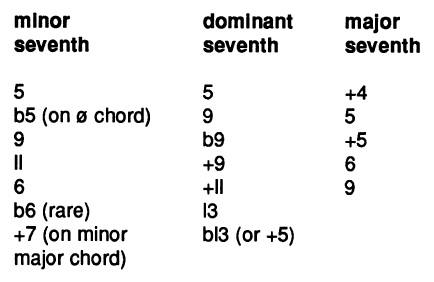
\includegraphics[width=3.1in]{levineextensions.jpg}
	\caption{Mark Levine's chart of possible additions to the common three-note seventh chord voicings.}
	\label{levineextensions}
\end{figure}
There are a variety of ways through which it might be possible connect this simple model to jazz performance data.  Translated into corpus-analytic language, these traditional chord-quality voicing rules can be tested against the data of the Yale Jazz MIDI Piano (YJaMP) corpus.\footnote{The YJaMP corpus currently consists of 128 MIDI transcriptions of live solo piano performances by New Haven jazz performers.  The corpus is still growing; to participate, email \href{mailto:andrew.d.jones@yale.edu}{andrew.d.jones@yale.edu}.}  An algorithm may look for root-third-seventh voicings (with various added tones) as signs standing for the seventh chords Martin places at the bedrock of jazz syntax.

In the presence of possible added tones, root determinations may be ambiguous or impossible to automate (or even hand-annotate consistently).  To sidestep this issue, I ask a simpler but analogous question: what chords occur in the YJaMP corpus which contain the three identifying chord tones listed above voiced in root-third-seventh ascending register within an octave?  For example, using a labeling system in which voicings are described by their semitonal distances above the bass note, what kinds of voicings contain $[0,4,10]$?

\begin{figure}
	\centering
	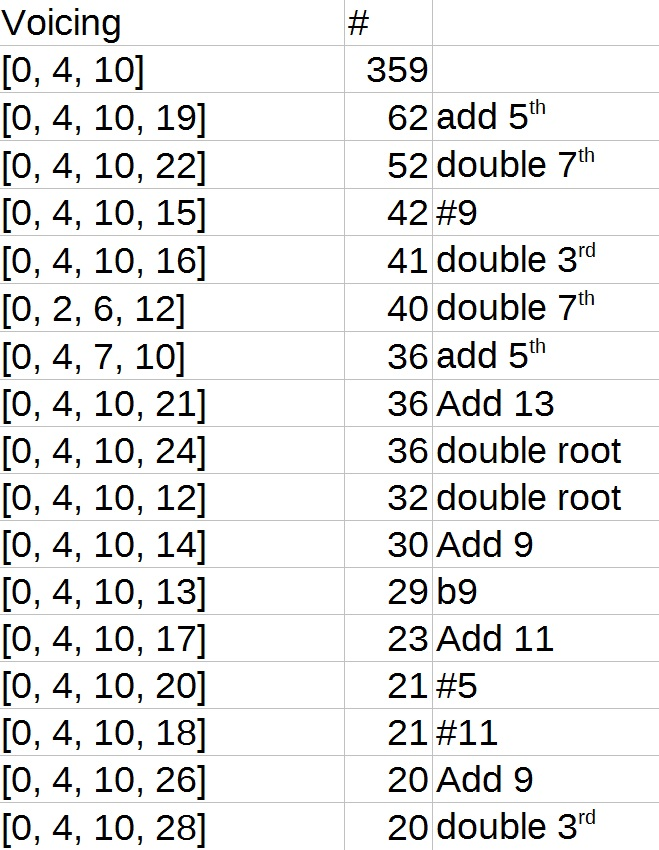
\includegraphics[width=2.7in]{0410_tones.jpg}
	\caption{Frequently-occurring corpus slices including $[0,4,10]$ voicing subsets.  These primarily include traditional dominant seventh chords with various added tones.  Note the unusual appearance of $[0,4,10,17]$.  On what basis do we teach students to ``avoid" this natural 11?  What is its nature?}
	\label{[0,4,10]}
\end{figure}

Figure~\ref{[0,4,10]} lists the most frequent voicings with dominant-seventh subsets.  To minimize reductive assumptions about non-harmonic tones, I search through ``salami slices" advocated by Quinn and White, na\"{i}ve verticalities agnostic about which pitches in a given stack should or can be disregarded.\footnote{For a full treatment of salami slice ideology, see Quinn and White [forthcoming].}  As an algorithm thinly ``slices" the YJaMP performance corpus, it tracks each appearance and disappearance of a pitch, treating each resulting verticality as a potential chord, regardless of its pitch content.\footnote{Ira Braus traces Quinn and White's usage of salami slices as musical metaphor back to comments by Ligeti; see Braus 2006.} take the term salami slice The most frequent chord additions match recommendations like those of Figure~\ref{levineextensions} almost precisely: chord tones like root, third, fifth, and seventh are added or doubled; diatonic extensions like 9 and 13 are added; alterations like $\sharp 9$, $\flat 9$, $\sharp 5$, and $\sharp 11$ are common.  The only place where the table of common voicings appears to disagree with received wisdom is in the frequent appearance of $[0,4,10,17]$, an apparent natural 11 chord.

Levine, among many others, advocates against such sonorities.  Giving an explicit reason to discount this ``unusual" chord (but frequent slice) requires a kind of two-step ideological appeal to reduction like the following:
\begin{enumerate}
	\item This chord contains a dissonant or quality-ambiguating minor 9th between its third and eleventh, rendering it problematic and giving it some kind of unstable acoustical status.
	\item The chord cannot fulfill its usual harmonic function as is: instead, it likely functions as some kind of passing or neighboring chord in the context of a less-problematic, more-normative dominant sonority.
\end{enumerate}
A corpus-supported analog to step (1) is unclear, and it would likely fall prey to Gjerdingen's analyst-bias objections.  Claims of problematic consonance and dissonance would require psycho-acoustical modeling, appealing to measurable properties of sounded chords and human responses to them.  Such studies are more common in the classical literature, but some jazz work in this direction has begun to appear.\footnote{Give some canonical examples like Krumhansl, but also jazz examples  like McGowan.}  Any corpus analytical claim regarding the impact of acoustical consonance on chord usage, if not accompanied by psycho-acoustical justification, would encode the analyst's expectations regarding jazz syntax into the data selection process, biasing any results meant to indicate how voicings appear in the corpus.  Pitch-based corpus statistics regarding which voicings are most common or important cannot be filtered for psycho-acoustic properties without biasing the results toward the whatever preconceptions the analyst chooses to encode.

A corpus of performances can be made to suggest lines of reasoning like (2); a tally of what kinds of voicings tend to follow $[0,4,10,17]$ provides a cursory suggestion as to its use.  If this voicing tends to progress to subsequent harmonies in a way strongly similar to (or different from) other dominant voicings, it may (or may not) stand in for Martin's dominant seventh chord category, despite Levine's intervallic contraindications.

Figure~\ref{[0,4,10,17]} shows the most common voicing salami slices to appear within 50 slices of $[0,4,10,17]$.  Each destination slice is indexed by both its semitonal voicing structure and the number of semitones its bass lies above or below the bass note of $[0,4,10,17]$.  For example, the most common nearby destination slice is the voicing $[0,1,5]$, the seventh, root, and third of a major-seventh chord in registrally-ascending order (see the yellow line in Figure~\ref{[0,4,10,17]}). The seventh of this destination chord (found in the bass) lies a major third above the bass of the preceding $[0,4,10,17]$ chord.  While the slice counting algorithm has made no assumptions of any kind about key, this ``progression" implies traditional root motion down by fifth, indicating that $[0,4,10,17]$ most frequently appears in the context of dominant-tonic motion.  Crucially, this dominant-tonic motion typically occurs on a time scale of many (18-30) slices; during that span, the ``unusual" voicing has plenty of opportunities to ``resolve" to a more normative dominant-seventh, like $[0,4,10,14]$, or a consonant dominant triad, like $[0,16,19]$ (see the blue line in Figure~\ref{[0,4,10,17]}).  Due to the wide variety of destination voicings found after $[0,4,10,17]$, this is comparatively weak support for the two-step reduction outlined above, but it does indicate the form such an appeal might make in corpus analytic terms.

\begin{figure}
	\centering
	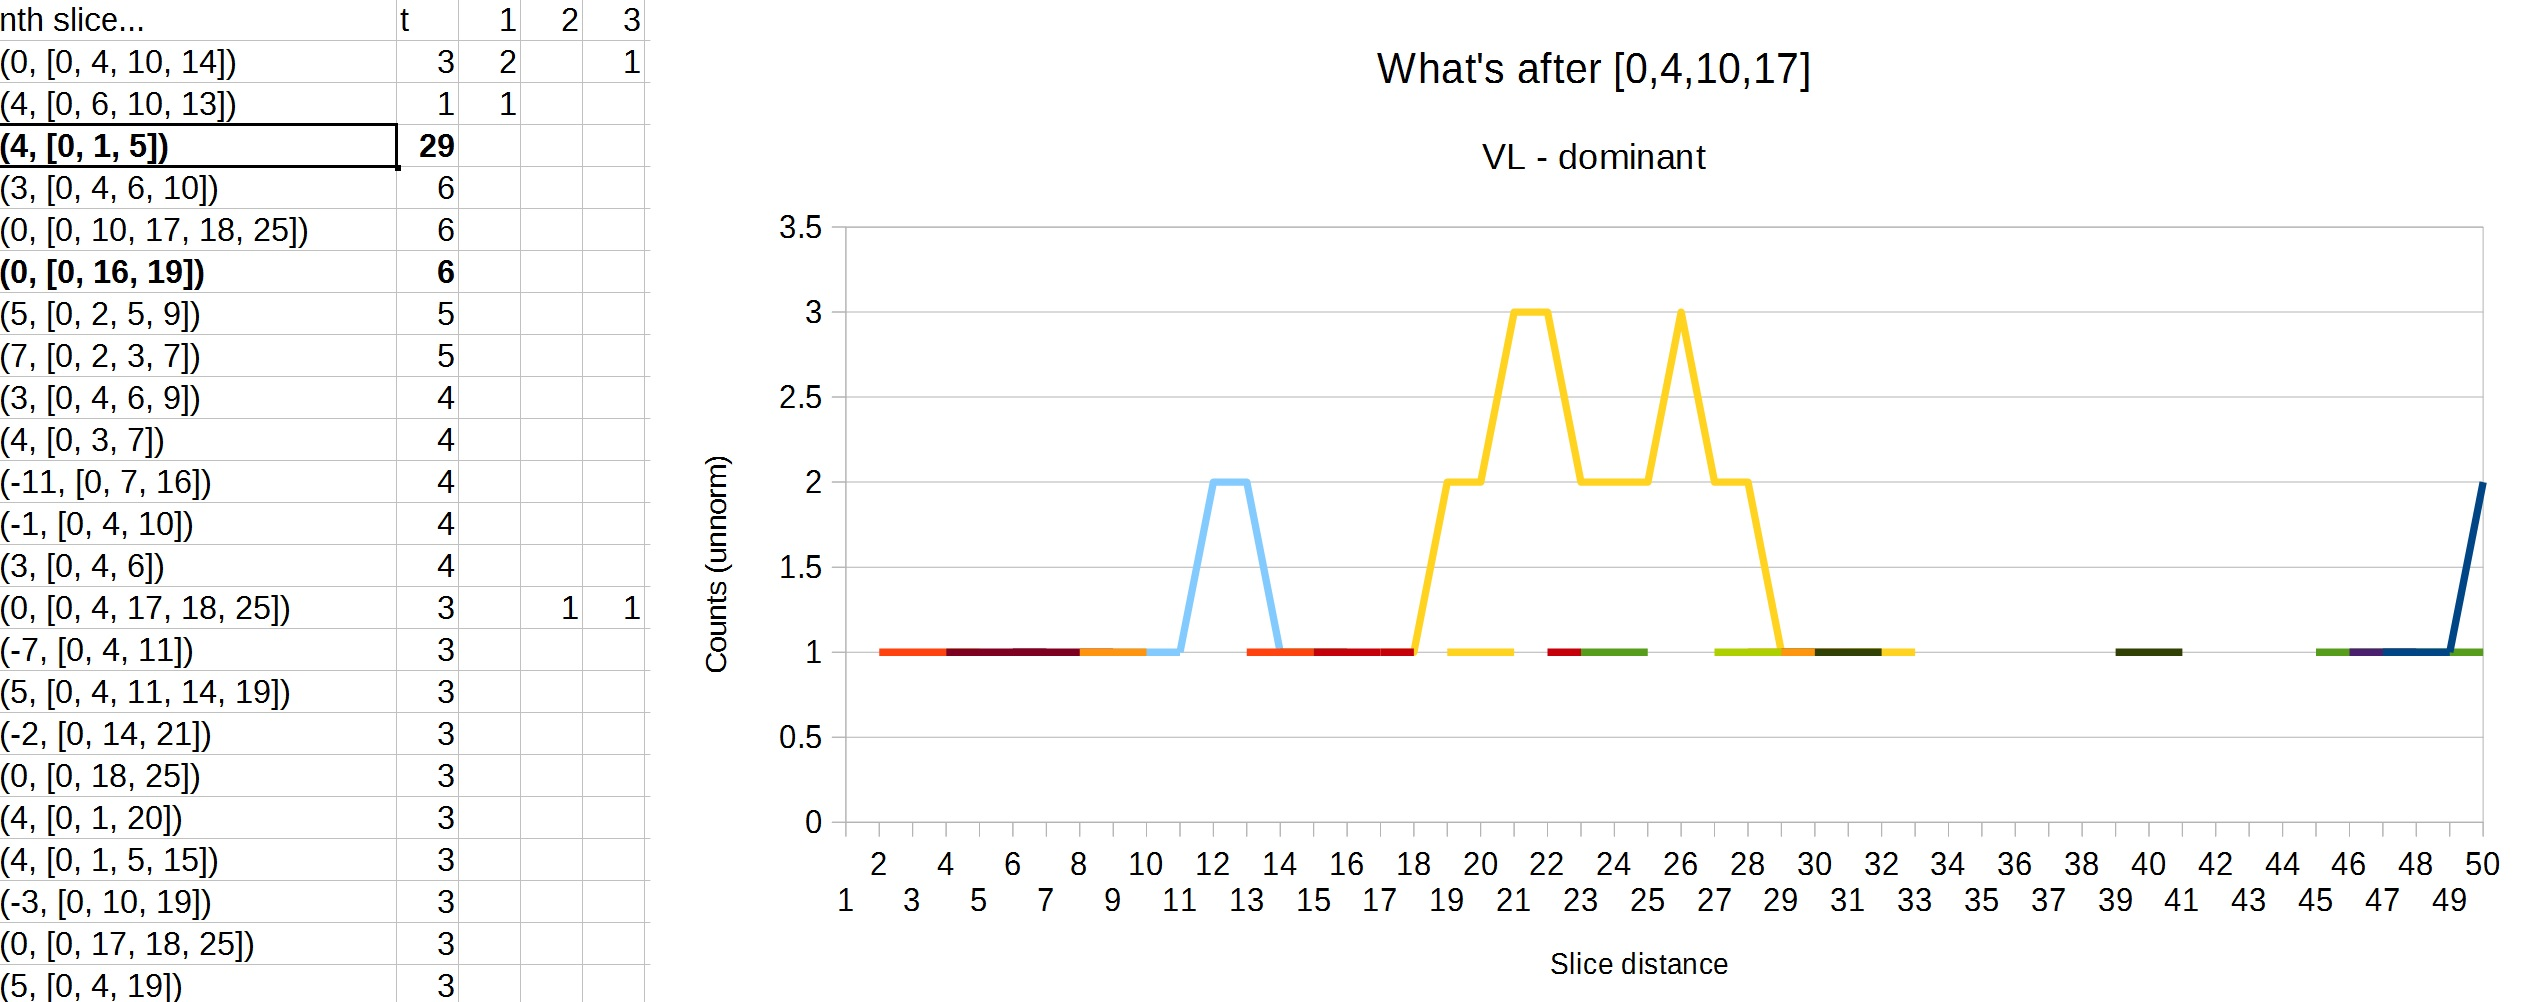
\includegraphics[width=6.5in]{041017_behavior.jpg}
	\caption{Following slice behavior for $[0,4,10,17]$ voicings.  The voicing appears most frequently in the neighborhood of $[0,1,5]$ voicings a major third up (yellow line), implying its participation in dominant progressions.}
	\label{[0,4,10,17]}
\end{figure}

%TODO: consider if fuller slice statistics go here, or later?

This procedure relies on a particular type of descriptive and explanatory model, and it still encodes analytical (and ontological) preconceptions regarding chord structure and harmonic progression.  To produce claims of this kind, there must exist a small number of frequently-employed chords of some ideologically-approved structure (i.e., seventh-chords with approved extensions and alterations) and a set of reduction techniques designed to render sounding sonorities of other types analytically (or at least syntactically) unimportant.  As the next section demonstrates, the assumptions of this selection process map onto a flexible semiotic structure given by Paul Kockelman. 

\section{Selecting Objects of Harmonic Significance}
%Introduce and unpack Kockelman's semiotic diamond
The analytical pathway from abstract seventh chords to actual voicing statistics given in the preceding section relies on a selection process similar to those captured by Kockelman 2012 in his Figure 2.6, reproduced as Figure~\ref{kockelman} below. 

\begin{figure}[h]
	\centering
	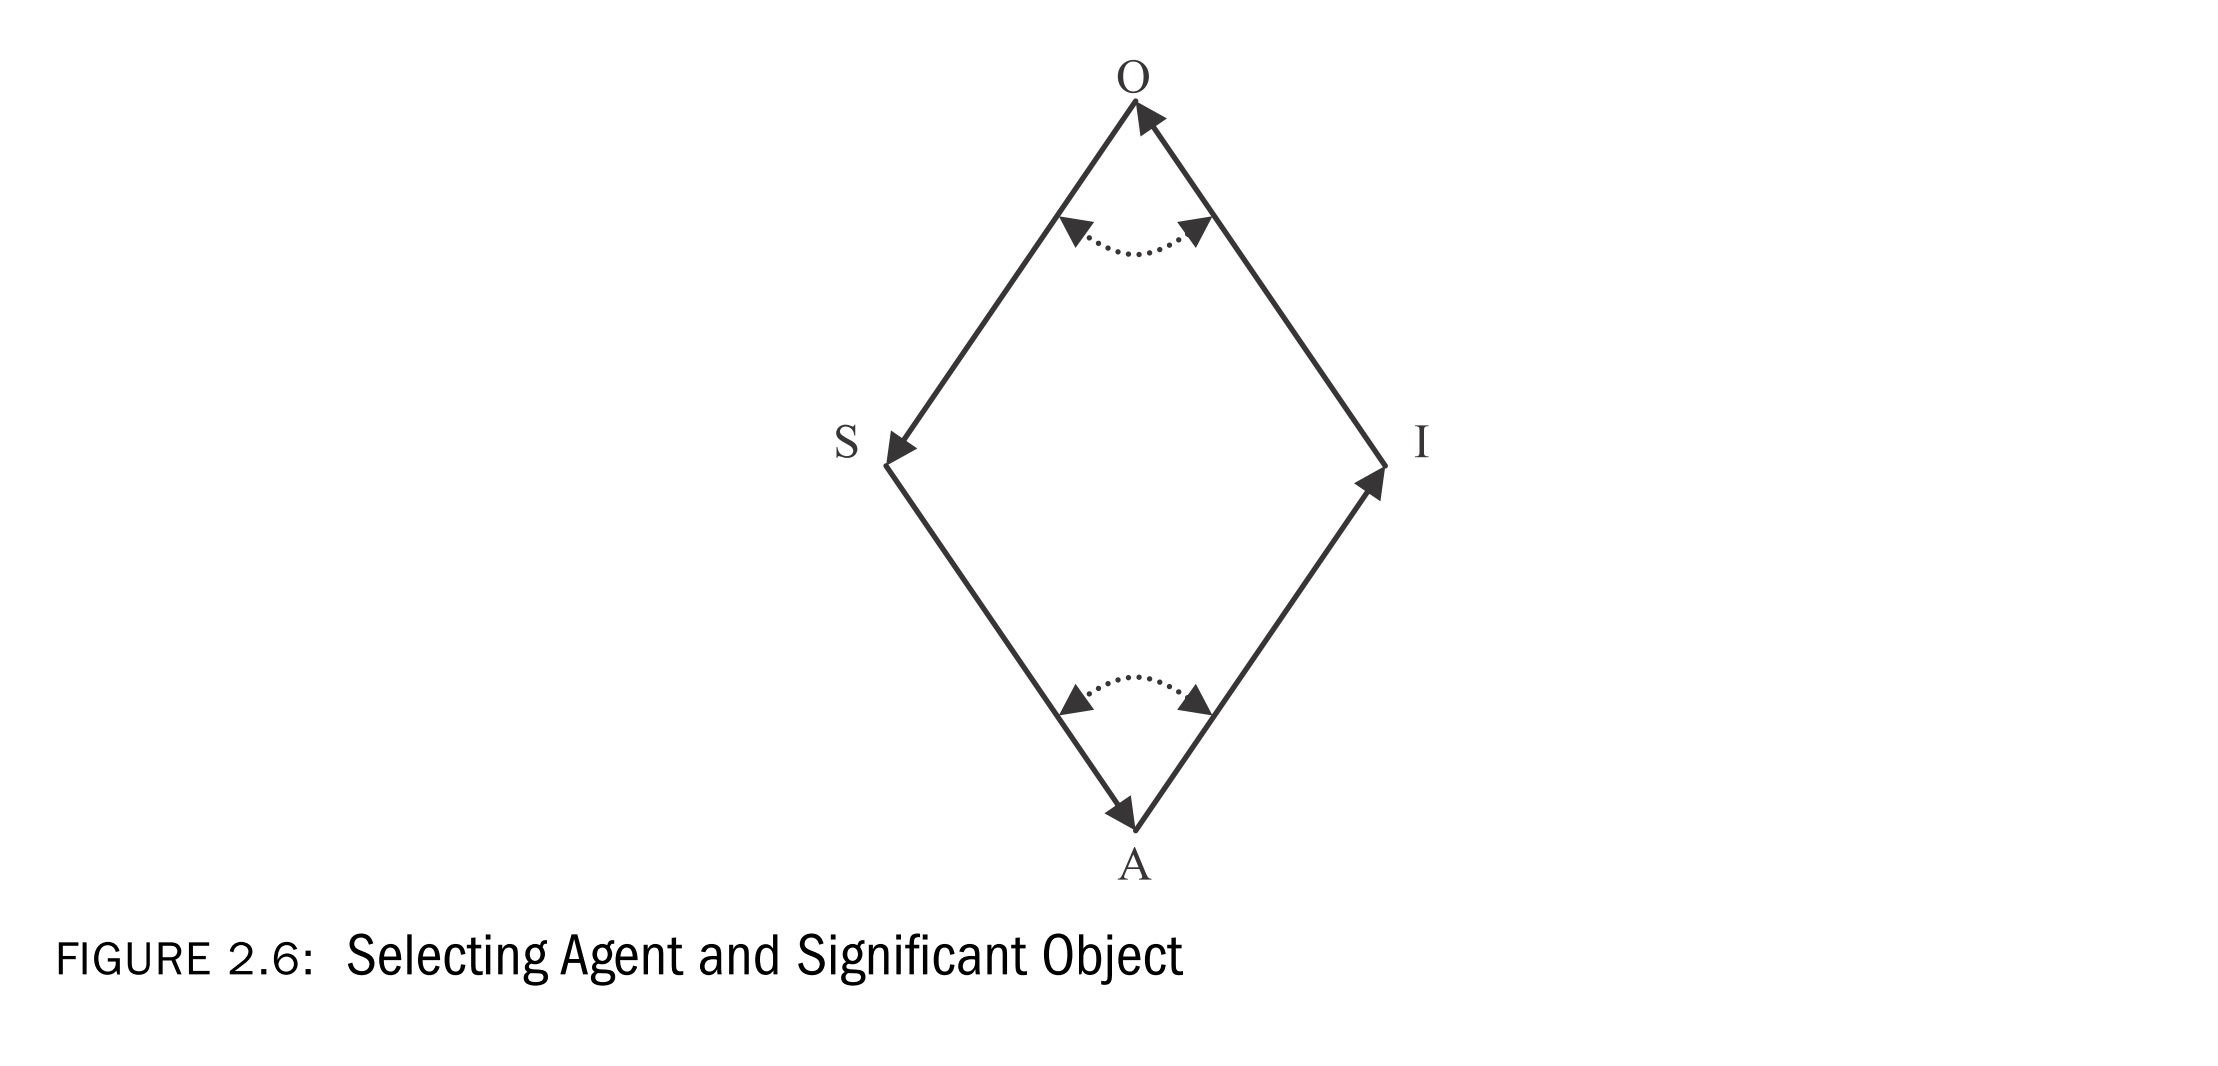
\includegraphics[width=6in]{kockelman_model.jpg}
	\caption{Figure 2.6 from Kockelman 2012, a general model for the ``relation between relations" inherent in selection.  The significant object (O) and selecting agent (A) are codetermined by their relations to observable signs (S) and resulting interpretants (I).}
	\label{kockelman}
\end{figure}

At the top and bottom corners of this diamond, such music analysis places the abstract chord objects ($O$) postulated as harmonic categories (like Martin's ontologically-basic seventh chords) and the analytical agent seeking to identify, transform, and react to those objects ($A$).  The analyst does not observe the postulated objects directly, but rather through certain traces or signs ($S$) found in the performance data, be it acoustical (for a listening agent or pianist), visual (for a score analyst), or digital (for a corpus analyst).  The analyst observes these signed traces and produces interpretants ($I$) that make sense given the presumed existence of $O$.  These interpretants might be roman numerals that an analyst assigns to particular sonorities to represent the category of harmonic object to which they belong, or they may be expectations regarding subsequent objects which might be sounded in a performance, among other possibilities.

In a very basic analysis, the analyst might encounter a root-third-seventh voicing like $[0,4,10]$ and interpret it as a sign $S$ for an abstract ``dominant seventh chord" object $O$.  The analyst might then apply a roman numeral interpretant like $V^7$ to a particular location in the score and begin looking for the next syntactically-appropriate chord.  For Kockelman, the interpretant ``makes sense in the context of $S$ from the standpoint of $A$."\footnote{Kockelman 2012, p.\ 17.}  The agent/analyst $A$ selects certain indices $S$ by turning signs into actions.  But Kockelman also describes the properties of the \emph{object} through a parallel and codetermined process: just as the interpretant $I$ makes sense from the standpoint of $A$ in the context of $S$, ``$I$ makes sense in the context of $S$ given the properties of $O$."  The resulting ``relation between relations" underpins semiotic processes of selection and significance, since the sense-making of $I$-given-$S$ requires and produces both a selecting agent and a significant object -- though the ontological structure from which the object $O$ arises can only be accessed, described, or interpreted by $A$ indirectly, through actions based on signs.

The flexible framework of Figure~\ref{kockelman} applies to a huge variety of selection processes, including many contexts where musical actions are taken.  In the case of actual performance, a jazz vocalist may interpret heard sonorities $S$ as indicating that a pianist is playing a kind of dominant seventh chord object $O$, and the vocalist might then choose to sing certain notes well-suited to that chord and expect and prepare for certain kinds of (say, tonic) sonority to sound after a particular time delay.  The fact that these actions make sense from the perspective of the singer (given the original heard sonority) is thoroughly entangled with the fact that the resulting actions make sense with respect to the properties of $O$ given the presence of $O$'s significant indices $S$.

Crucial to Kockelman's description of selection and significance is the claim that all agents performing (re)actions \emph{must do so under some ontological assumptions}, whether they are conscious or unconscious, enminded or embodied.  For an analyst to assign a roman numeral to a sonority, the analyst must partake of an ontology in which a variety of sonorities map to each roman numeral on the basis of their pitch class content as tokens of a type or individuals of a kind.  The analyst's interpretant (i.e., ``$V^7$," or ``look for a subsequent tonic") makes sense if and only if the kind ``dominant seventh chord with a root on scale degree five" has properties underpinning the identification of sonority/sign $S$. To use recursive language echoing Kockelman's own descriptions, the relation between the analyst-interpretant relation and the sign-analyst relation mirrors the relation between the interpretant-object relation and the object-sign relation.  Selecting a labeled kind correlated to a set of signed indices relies on and produces an ontological system.  

%Modes of ontological transformativity
Kockelman's careful attention to signed indices and acted interpretants as integral components of semiotic processes allows him to typologize their potential ontological impacts.  Consider three ``modes of ontological transformativity," to adapt part of Kockelman's typology to a music-analytical case:\footnote{The most direct analog to this discussion surrounds Table 1.2 in chapter 1 of Kockelman 2012.}
\begin{enumerate}
	\item The presence of certain notes in a voicing may change the analyst's ontological assumptions about what kinds constitute and apply to the individual sonority: ``The sign $[0,4,10]$ makes me think this sonority is a dominant seventh chord."
	\item The presence of certain notes in a very large number of similar voicings may change the analyst's ontological assumptions about what notes or intervals make up a particular kind: ``Many sonorities seem similar to $[0,4,10]$ in some important way but carry indices $[0,4,10,15]$, so perhaps a property of dominant seventh chords as a kind is that they may contain a $\# 9$ above the bass."
	\item The presence of certain unfamiliar voicings in frequent but unfamiliar patterns may change the analyst's assumptions about what voicings and harmonic objects make up a particular style or musical world: ``Many voicings do not neatly align with qualities of seventh chord, so perhaps seventh chords are not the objects (or are not the \emph{only} objects) I should react to or label."
\end{enumerate}
Transformations of type (1) here correspond most directly to undergraduate-style harmony assignments, where student analysts map observed traces to stable, received chord categories.  Transformations of type (2) constitute much of the academic music theory literature, where professional analysts logically induce pitch-based patterns of behavior from a particular corpus given a mostly-stable set of ontological kinds.  Both of these modes of ontological transformativity are well-suited to corpus analysis relaying on the ``numerical methods and explicit algorithms" Gjerdingen describes as appropriate for two-thirds of his recipe.  Gjerdingen's bias objection primarily concerns transformations of type (3), where the categories signed and represented by the statistically-tallied indices themselves change.  And the avoidance of such changes is impossible, since selecting agents produce and are imbricated in their own ontologies -- to get any selection and response procedure off the ground, the analyst must encode some set of ontological assumptions.  Where Gjerdingen says this reveals a ``presentist or historicist bias," we might say that this reveals the necessity (and inescapability) of ontological framing in analytical processes.

%aligning relations between relations
If the properties of the object and the actions of the agent are entangled across a semiotic process of selection and significance, the signed indices to which the agent reacts may be framed in a variety of ways; analysis will not consist of unearthing pre-existing harmonic objects, but rather of framing a harmonic ontology in which the properties assigned to chord objects align with the interpretants produced by the agent(s).  Different agent-interpretant relations -- different types of action or expectation taken or embodied by the analyst -- may relate more directly to certain kinds of object-sign relation than to others.  This alignment of relations between relations guides the framing of this dissertation and results in a close focus on the relays between computational category formation and temporal statistics.

\section{Harmonic objects and interpretants}
%lay out several analytical interpretants and the object-sign framings best related to them
Modes of harmonic analysis with different interpretants and objects can be framed accordingly.  Four are shown in Table~\ref{frames}.
\begin{table}[h]
  \caption{Four framings of harmonic analysis generating (and requiring) different semiotic ontologies.}
  \centering
\begin{tabular}{p{1.75in} |p{2in} | p{2in}}
\hline\hline
Interpretant & Signed Indices & Harmonic Object \\ [0.5ex]
\hline
Identifying a voicing structure & Intervals above the bass at a particular time & Pitch verticalities \\
Postulating a scale & Pitch class frequencies over time & Macroharmonic collections \\
Assigning a traditional roman numeral & Keys, pitch-class sets, reduction rules & Tertian scale degree stacks \\
%Choosing a key & Scales and articulated centricity & Tonics and modes \\
Interpreting a chord's syntactic function & Scale degree sets over time & Categories of similar scale degree sets \\[1ex]
\hline
\end{tabular}
\label{frames}
\end{table}
An analyst seeking to identify a type of voicing, following the directions of Martin and Levine, assumes (and produces) a class of pitch verticalities ($O$); the decision to place a given sonority into such a class (be they quality-based, cardinality-based, or otherwise) makes sense to the analyst given its intervals above the bass ($S$) and the existence of voicing classes ($O$) with certain intervals above the bass as properties.  This analytical process requires minimal temporal data, as the sonority's voicing structure can be gleaned from an extremely brief snapshot of a score or fragment of an audio recording, but it still assumes some temporal properties as the basis for its ontology: voicings as pitch verticalities are typically represented as simultaneities, when actual performance traces will surely exhibit slight onset time differences between each of the notes ``in" a voicing.

On another temporal scale, an analyst postulating a scale underpinning a certain passage of music assumes (and creates) limited macroharmonic collections of pitch classes that can be related to musical surface signs in particular ways; if pitch-class distributions can lead the analyst to produce a scale, then the scale object can be given such a surface distribution as a property or signed index.  In this case, as in the voicing case, the method by which the agent produces an interpretant from signed indices aligns with the properties assigned to the objects in the resulting semiotic ontology.

To assign a roman numeral or interpret a chord's syntactic function requires a more complex ontology, where the semiotic relations between the objects' properties and the agents' interpretants become less direct.  For a traditional roman numeral to ``make sense" to an analyst, she must postulate the existence of keys and pitch-class sets standing in some relation to one another.  To label the (untransposed) pitch class set $[0,4,10]$ as $V^7$ is also to assume (or create) a kind, ``$V^7$," connected to signed indices in some meaningful way.  The nature of this connection, the sense-making of ``$I$ in the presence of $S$ given the properties of $O$," is codeterminate with the with the sense-making of ``$I$ in the presence of $S$ from the perspective of $A$."  Put more provocatively, the precise way in which the analyst turns surface signs into interpretants (analytical symbols and expectations) may be thought to generate (and respond to) the way harmonic object categories relate to their signed indices (pitch and temporal properties).

On this basis, roman numeral analysis as an interpretive act fractures into several separate semiotic processes with their own distinct ontological conditions.  If the analytical interpretant produced ($V^7$) makes sense to analyst $A$ because it consists of a tertian stack of dominant seventh quality built on scale degree $\hat{5}$ of the local key, then the semiotic kind to which the individual sonority has been assigned carries properties based solely on its pitch class structure and relation to a key.  But if the same analytical interpretant is produced through some other relation to pitch and time indices, the kind $V^7$ may participate in an entirely different ontology permitting entirely different properties and modes of proof.  In particular, if $V^7$ makes sense to analyst $A$ \emph{because the observed sonority ``behaves like" other chords of kind $V^7$}, the ontological structure embedding the kind $V^7$ changes quite radically.  The relation between kind $V^7$ and its indices can no longer be captured by pitch class structure and key relation; instead, it requires additional -- and potentially conflicting -- knowledge about temporal progression or syntactic function.  As the last line of Table~\ref{frames} indicates, the interpretation of a chord's syntactic function treats more than a sonority's pitch structure as indices; such an interpretant also involves the agent's knowledge regarding what chords tend to succeed the given sonority at certain time scales.

The same human analyst may produce interpretants over-determining the properties assigned to harmonic categories at various levels of ontological transformativity.  Observing a chord's pitch-class structure or that it almost always precedes a stable tonic might lead the analyst to recognize it as part of the kind $V^7$, an ontological transformation of mode (1) above.  Or the repeated observation of those indices might lead the analyst to decide that they stand as properties of the kind $V^7$, a mode (2) transformation.  Or the analyst's concern that many chords which display some of the expected indices but not others (say, common progression behavior but unfamiliar pitch class structure) might lead to a re\"{e}valuation of the ontology framing the kind $V^7$, producing a kind category at a higher (or overlapping!) ontological level like ``dominant function," where progression behavior constitutes the signed indices producing interpretants, relegating exclusively pitch-structural indices to kinds like $V^7$.  In such an ontology, interpretive acts like ``this chord is a $V^7$" and ``this chord has dominant function" would partake of separate ontologies, rely on distinct types of evidence, and involve different analytical skills.

%transition to particular corpus-analytical harmonic analysis framings.
Some of the most-maligned limitations of computational methods -- their blessed ignorance of musical context and their blind reliance on the digital representation of the corpus -- can prove crucially useful for the generation of particular and consistent semiotic ontologies.  While human-generated interpretants like ``this sonority is a $V^7$" or ``this chord typically precedes tonic" can reference categories over-determined by their relation to indices of varying modality, algorithmic statistics and machine learning methods can be forced to produce interpretants which make sense only and precisely in the context of particular sets of indices.  With a Python implementation of an algorithm as agent $A$ in Figure~\ref{kockelman}, the direct relation between the sense-making of $I$ in the presence of $S$ from the perspective of $A$ and the sense-making of $I$ in the presence of $S$ given the properties of $O$ is strictly enforced.  The algorithm can only assign properties to object categories based on the input indices it observes -- it knows no other possible features of the object than the signs encoded in the corpus's representation.  

The remaining sections of this chapter provide examples for how such algorithmic work might ``object"-ify the YJaMP corpus.  Given interpretants designed to operate at different time scales and with different analytical aims, different computational processes are employed to ensure that the interpretant-agent-sign relations are precisely co-generated with the interpretant-object-sign relations.  The categories used to describe harmonic objects in the corpus generate different ontologies in different analytical circumstances.  Statistics regarding voicings and scales suggest future analytical projects based on YJaMP or other corpora, while temporal encodings of scale degree sets lay the groundwork for the generalized harmonic progressions of chapter 3 and the syntactic category formation of chapter 4.
 
\section{Voicings revisited}
%TODO: salami slices, voicings in general, now with a touch more ontology?

[Note: Figure~\ref{[0,4,11]} and Figure~\ref{[0,3,10]} provide voicing statistics for major and minor seventh chords, but the results are trickier to interpret than those for $[0,4,10]$.  I include them below, and we can talk about them in colloquium if people are interested.]

\begin{figure}[h!]
	\centering
	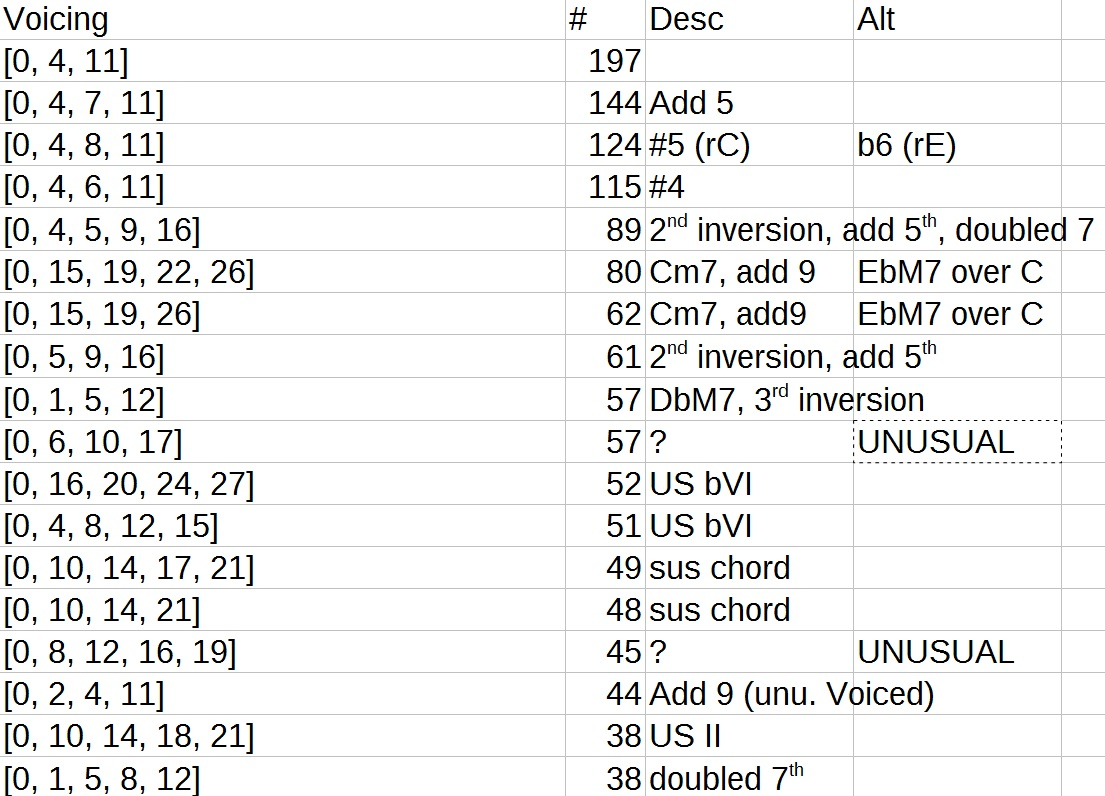
\includegraphics[width=5in]{0411_tones.jpg}
	\caption{Frequently-occurring corpus slices including $[0,4,11]$ voicing subsets.  These include traditional major seventh chords with various added tones, but also other traditional (``sus") and non-traditional ($[0,6,10,17]$) chords.}
	\label{[0,4,11]}
\end{figure}

\begin{figure}[h!]
	\centering
	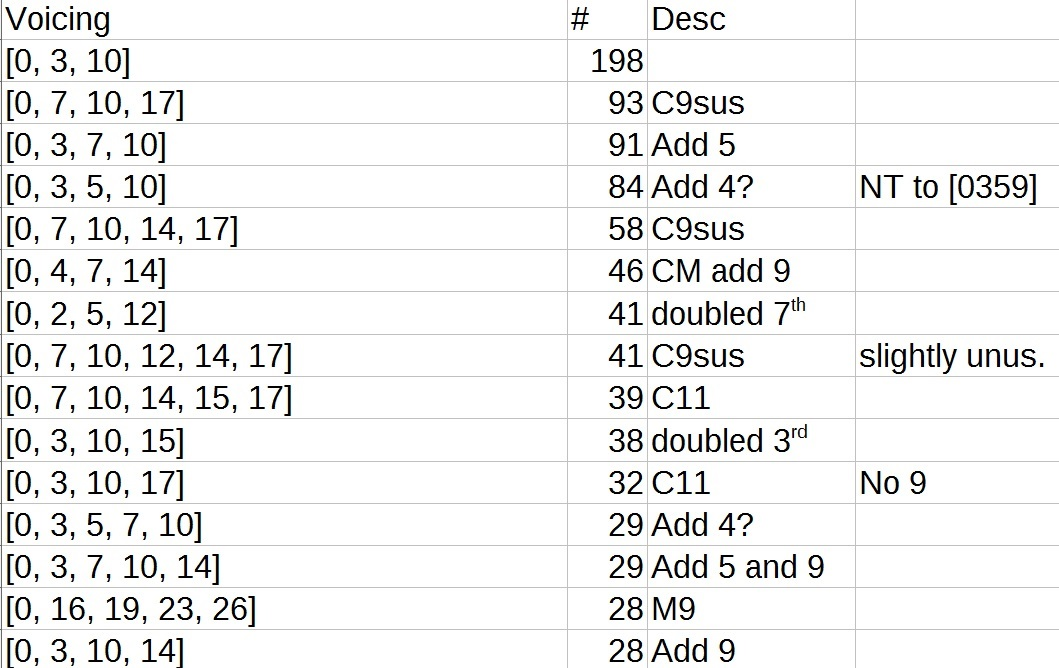
\includegraphics[width=5in]{0310_tones.jpg}
	\caption{Frequently-occurring corpus slices including $[0,3,10]$ voicing subsets.  These include traditional minor seventh chords, with various added tones, as well as several voicings of ``sus" chords.}
	\label{[0,3,10]}
\end{figure}
\newpage


%TODO: what good does this do in the new chapter structure?  Re-write or cut
Tallying unfiltered, unaltered salami slice voicings produces two immediate problems.  First, the most frequent slices contain just one or two pitches and are unlikely to provide useful harmonic information.  Second, there are thousands of different voicing structures in the YJaMP corpus alone, even if each one is only indexed by the semitonal distances above its bass note.  In an attempt to mitigate both of these problems, I use a hybrid pitch/pitch-class scheme: each slice is indexed by a set of pitch classes corresponding to chromatic scale degrees as well as the scale degree found in the bass.  As a first pass, I assign a single key to each jazz track using the Bellman-Budge weightings for a Krumhansl-Schmuckler key determination algorithm.\footnote{I'd like to upgrade to local window keyfinding, but that's not quite ready.}  Within each track, I then have Python/Music21 label each slice in the key's coordinates -- for example, first-inversion tonic triads would be given the label $([0,4,7],4)$.  

This voicing-to-scale-degree-set reduction process does not help the fact that small-cardinality slices dominate the data.  To draw high-frequency chords out of the slices, I turn to superset relations.  First, I assemble a unigram probability table for all the slices in the corpus.  Next, I make a second pass, comparing the unigram probability for each given slice of cardinality greater than one with the unigram probabilities for each chord present in the corpus of which the slice is a pitch class subset.\footnote{The code does not address slices of cardinality one, as each such slice would be a subset of all possible pitch class sets.}  The slice is counted in the category of its most probable superset.

This has the attractive feature of enforcing a kind of balance similar to the accuracy-simplicity trade-off described above.  Small-cardinality slices tend to occur more frequently in the corpus, but they have fewer subsets to contribute counts; large-cardinality slices occur less frequently in the corpus, but they tend to have a larger number of subsets, each of which might contribute counts to the category tally.  As a result, the table of most frequent superset slices seen in Figure~\ref{supersets} represents a data-driven, pragmatic middleground, an appropriate scale at which to suggest a trade-off between large-vocabulary coverage and small-vocabulary generalization.  Dyads built on prominant scale degrees appear high on the list, as do chords corresponding to $Dm7$, $FM7$, and $CM7$ (relative to $CM$).  A variety of other chords with traditional tonal structures appear lower in the list, including a variety of dominant chords with extensions.
\begin{figure}
	\centering
	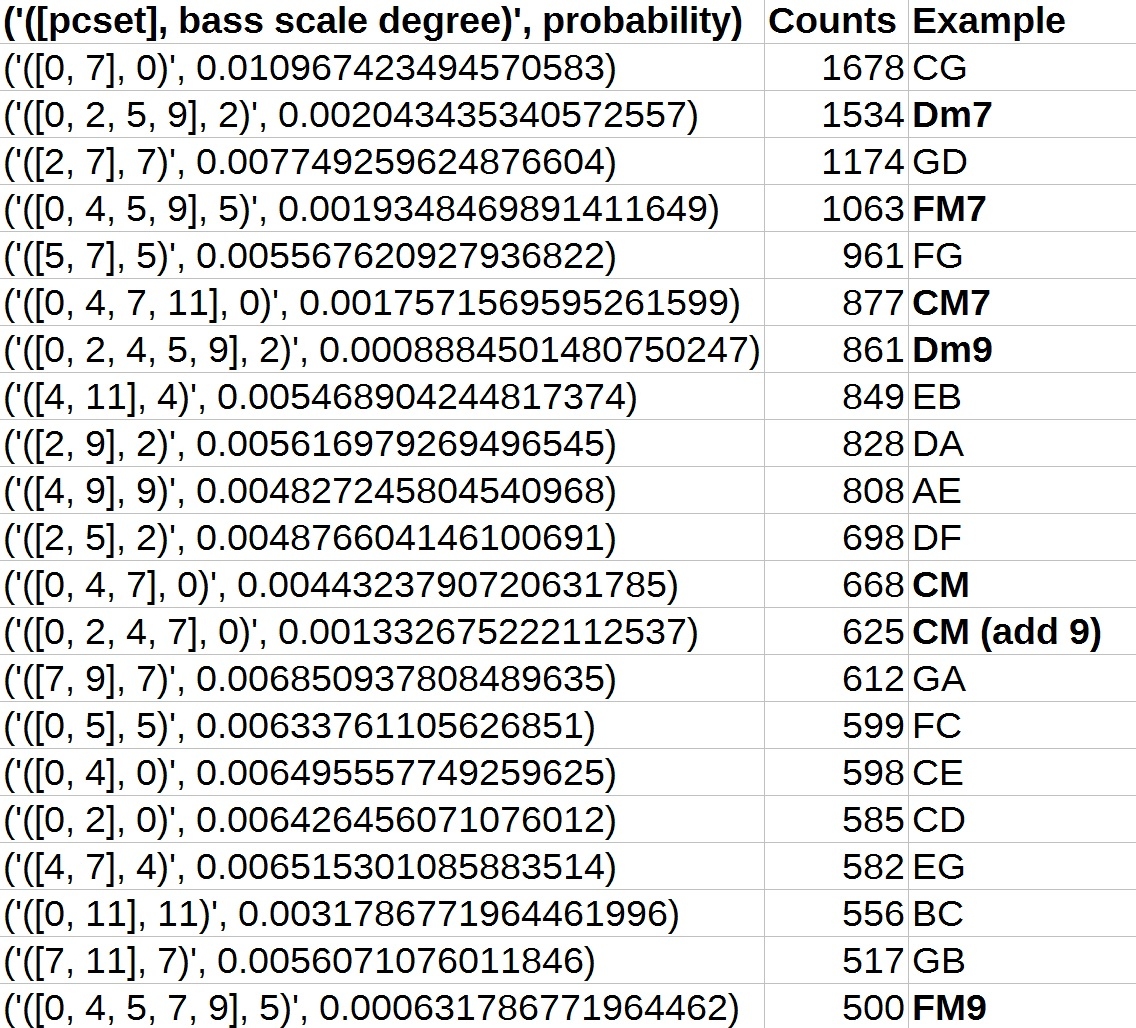
\includegraphics[width=5in]{pc_slice_supersets.jpg}
	\caption{A tally of slices in the jazz piano corpus categorized by the most corpus-probable member of a given pc-set's superset tree.}
	\label{supersets}
\end{figure}

It is worth noting that this unremarkable list makes no assumptions about chord structure, consonance, or cardinality.  Dissonant slices are treated exactly the same as perfect fifths, and dyads start on the same footing as pentatonic scales, stacks of fourths, and seventh chords.  No reduction of non-harmonic tones has been employed.  The fact that minor, major, and dominant seventh chords of cardinality three, four, and five appear on the list anyway indicates that postulating these chord qualities as important harmonic categories is well-supported in the YJaMP corpus.  Na\"{i}ve slice data suggests that traditional jazz-analytic categories can be shown to refer to objects with important ontological status.

\section{Chords as Local Macroharmonic Clusters}
%TODO: re-make this about long-duration scale-type interpretants
If triads and seventh chords of cardinality three, four, and five occupy a special status as appropriate representative slice categories in the corpus, it may be possible to find and make use of them while relaxing one further pillar of chord identity: instead of requiring that chords be some kind of verticality, we might ask if ``chords" can satisfy analytical functions without needing to be vertical in the first place.  It seems to me that chords serve three important purposes:
\begin{enumerate}
	\item They give us a sense of how we should expect nearby notes to behave, as well as of which notes we should expect to appear most frequently.
	\item They provide an indication of where in a phrase we are, often serving as a means of tune identification in the absence of melody.
	\item They orient us relative to a(n at least local) tonic/key.
\end{enumerate}
None of these require that chords be perfectly vertical stacks of notes, provided some localization criteria can be given.  Since the YJaMP corpus consists of MIDI data taken from real-time performances, I can partition the entire corpus into time-windows of small and equal size.  Within each window, I tally up the number of milliseconds each pitch class sounds.  The full set of durationally-weighted pitch-class vectors can be fed into a variety of clustering algorithms.  The optimized clustering prototypes provide a variety of objects for analytical inquiry relatively free from chord-structural assumptions.

The best results produced by an algorithm so far come from spherical k-means, a routine which uses a cosine metric to cluster pitch-class vectors with similar directions in 12-dimensional space.  All the user needs to specify is the desired number of clusters.  As the number of clusters increases, the accuracy of the clustering increases, but so does the complexity of the model.  For each given time window size, the clusters found tend to display cardinalities near the center of the ranges given in Figure~\ref{cardinalities} -- longer time windows tend to have a larger number of pitch classes in them.  Accordingly, an excavation of jazz chord objects in the corpus can proceed along the following pathway:
\begin{enumerate}
	\item Choose the time scale over which harmonic inquiry is to proceed.
	\item Examine the cardinality distribution for pitch-class sets of that window size.
	\item Choose a number of clusters such that the resulting cluster prototypes have cardinalities which represent the window size well.
\end{enumerate}
Sample results for windows of size 400ms, 800ms, and 1600ms are given below (in Figure~\ref{400clusters}, Figure~\ref{800clusters}, and Figure~\ref{1600clusters}).  In the 400ms windows, objects of cardinality three occur relatively frequently, many of which match traditional chord types.  Cluster prototype cardinalities increase in size for windows of 800ms and 1600ms; in the latter, many clusters better represent traditional scales than chords.  In each case, descriptive statistics generate a series of harmonic objects from the data without choosing chord types, consonances, or even verticalities in advance.

What is not clear, yet, is whether seeing traditional objects of inquiry in the results is sufficient to indicate that the corpus methods are a useful basis around which to build a harmonic ontology.  If weighted pc-set clustering only produces some of our boring preconceptions alongside some junk, then I should reconfigure what I think my methods can do for me; if, on the other hand, this type of clustering proves an acceptable means of pulling harmonic objects from noisy data, then corpus analysis should be able to take steps toward addressing Gjerdingen's object-first bias problem -- and it should be possible to do so with \emph{any} noisy corpus.

\section{Scale-degree sets and temporal progressions}
%TODO: set up chapter 3 by giving some ontology and statistics regarding the sd-sets that will come up?

%look at what objects fall out from clustering at various time scales

\begin{landscape}
\begin{figure}
	\centering
	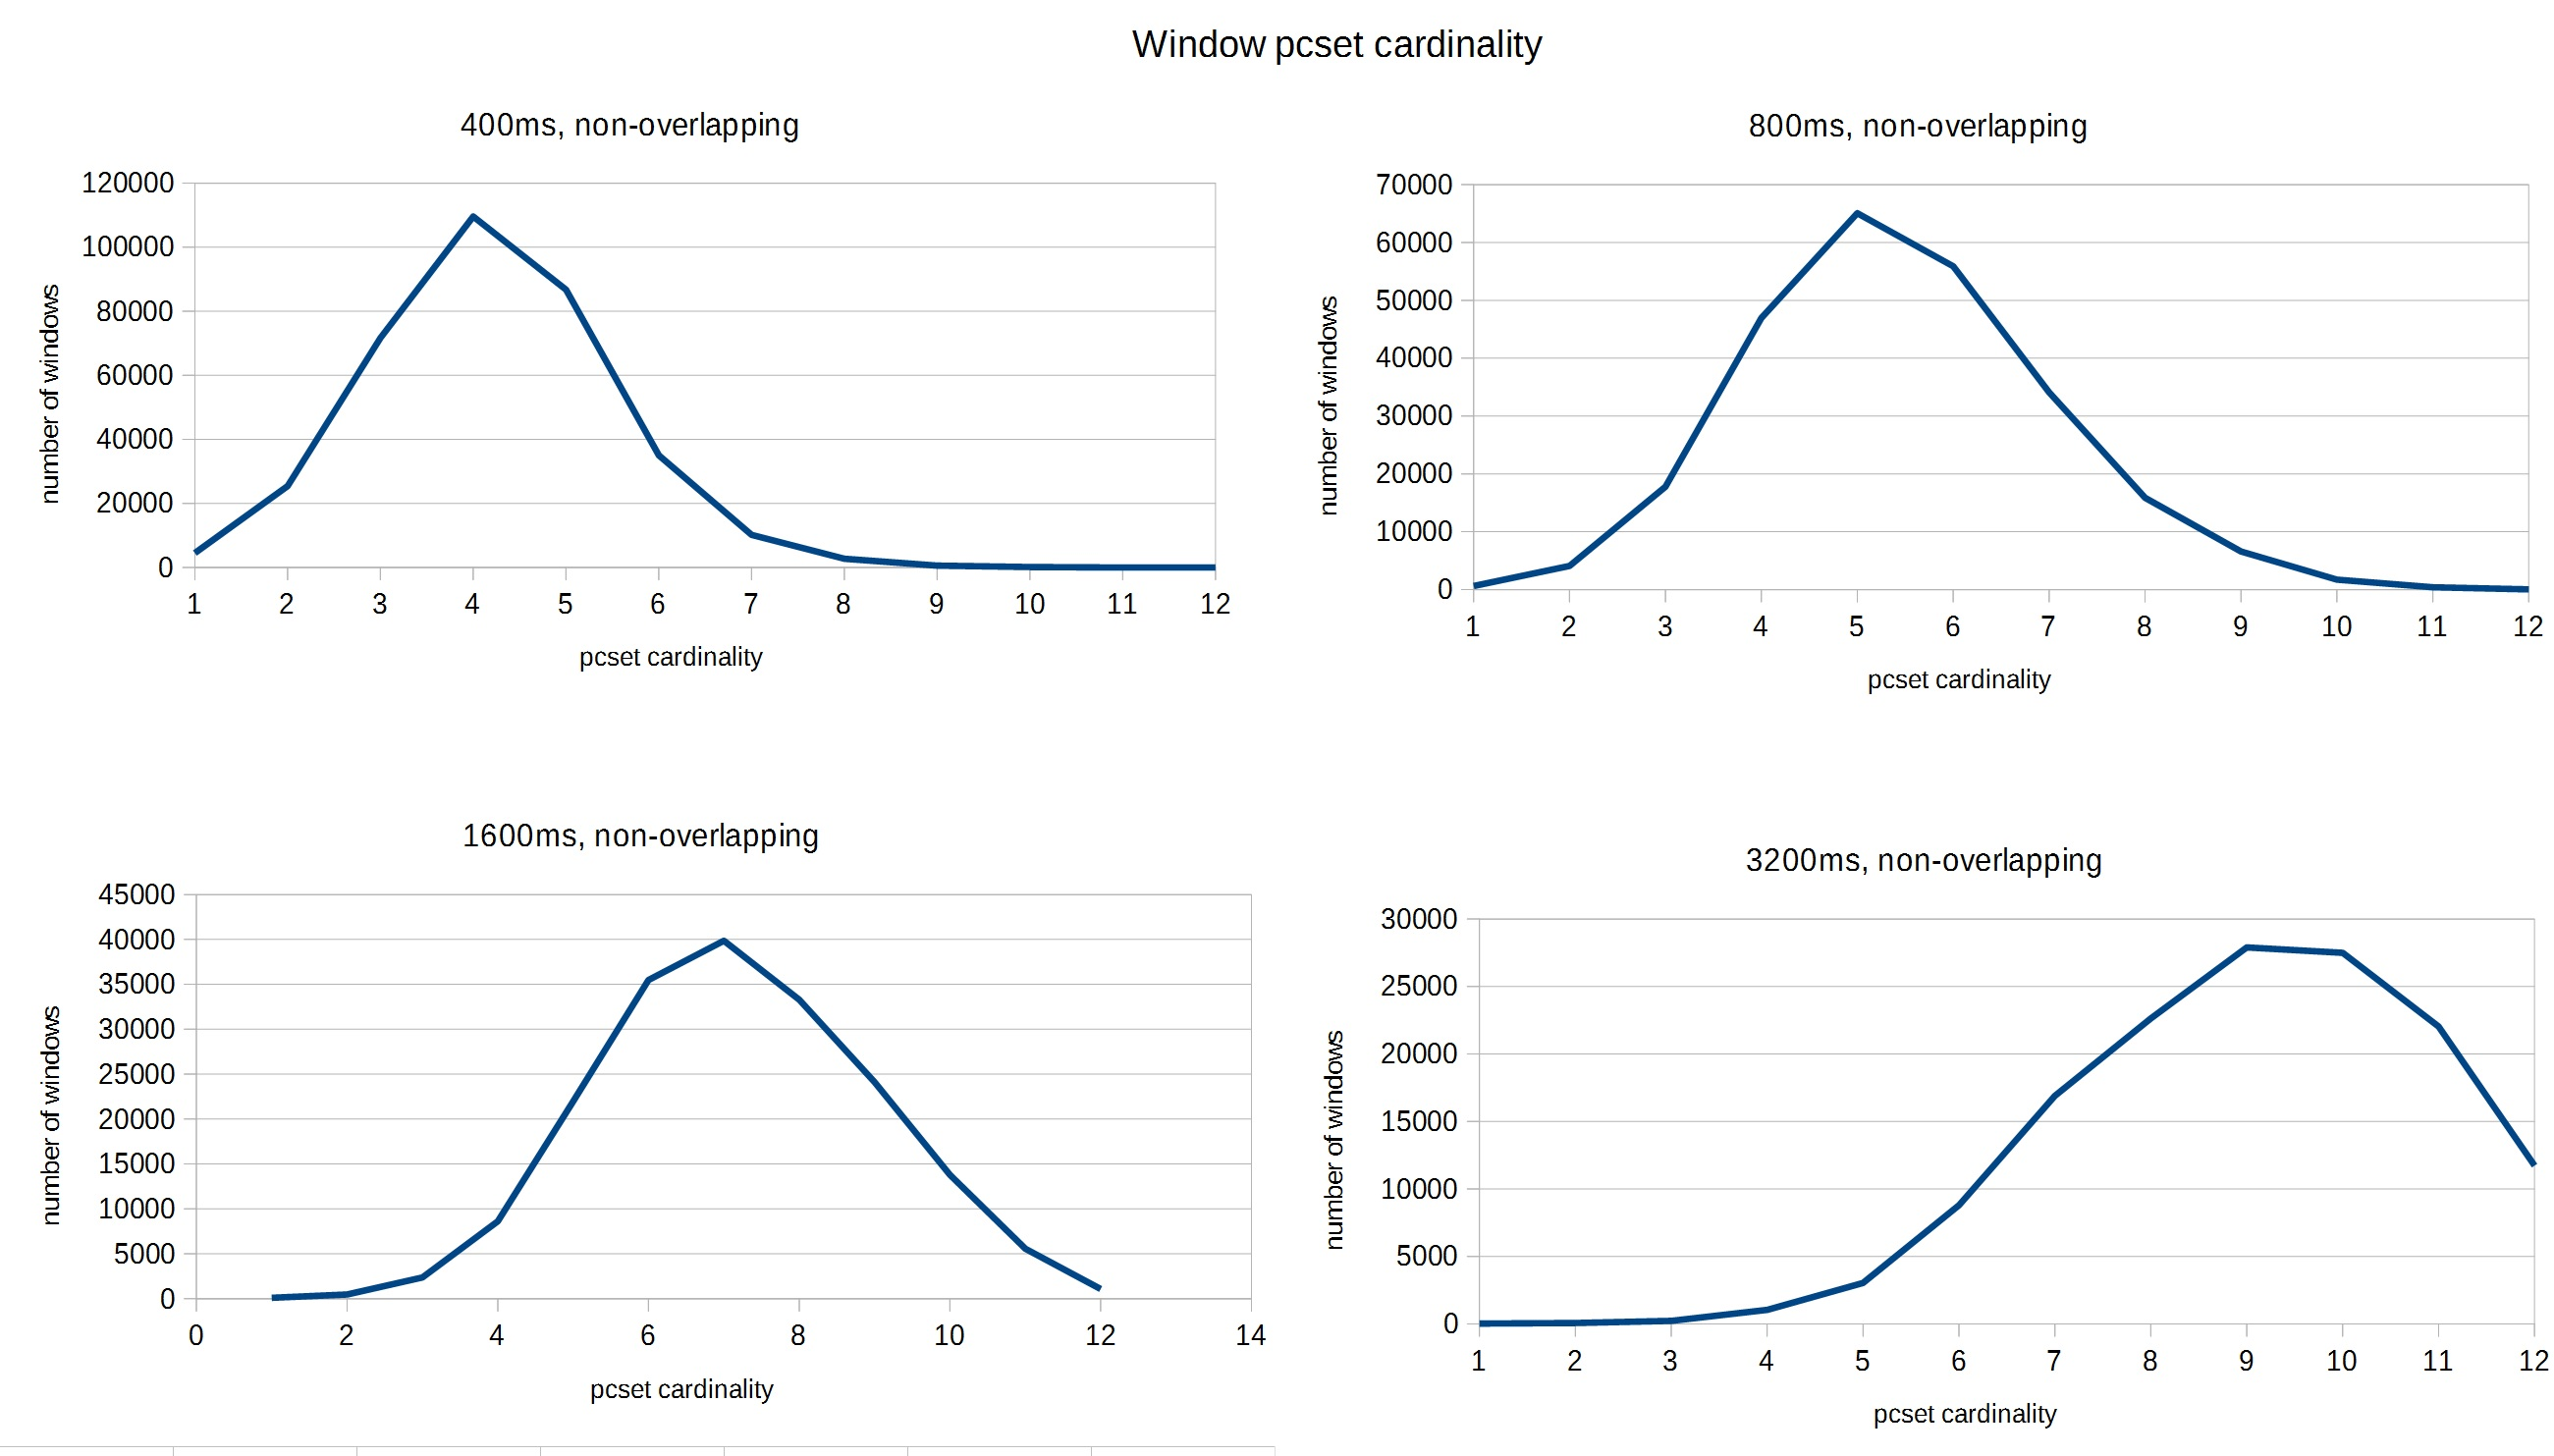
\includegraphics[width=8in]{cardinalities.jpg}
	\caption{Average pc-set cardinalities for four window sizes.  As window size increases, so does average cardinality; the time scale under examination is interrelated with the type and size of the resulting objects.}
	\label{cardinalities}
\end{figure}
\end{landscape}


\begin{figure}
	\centering
	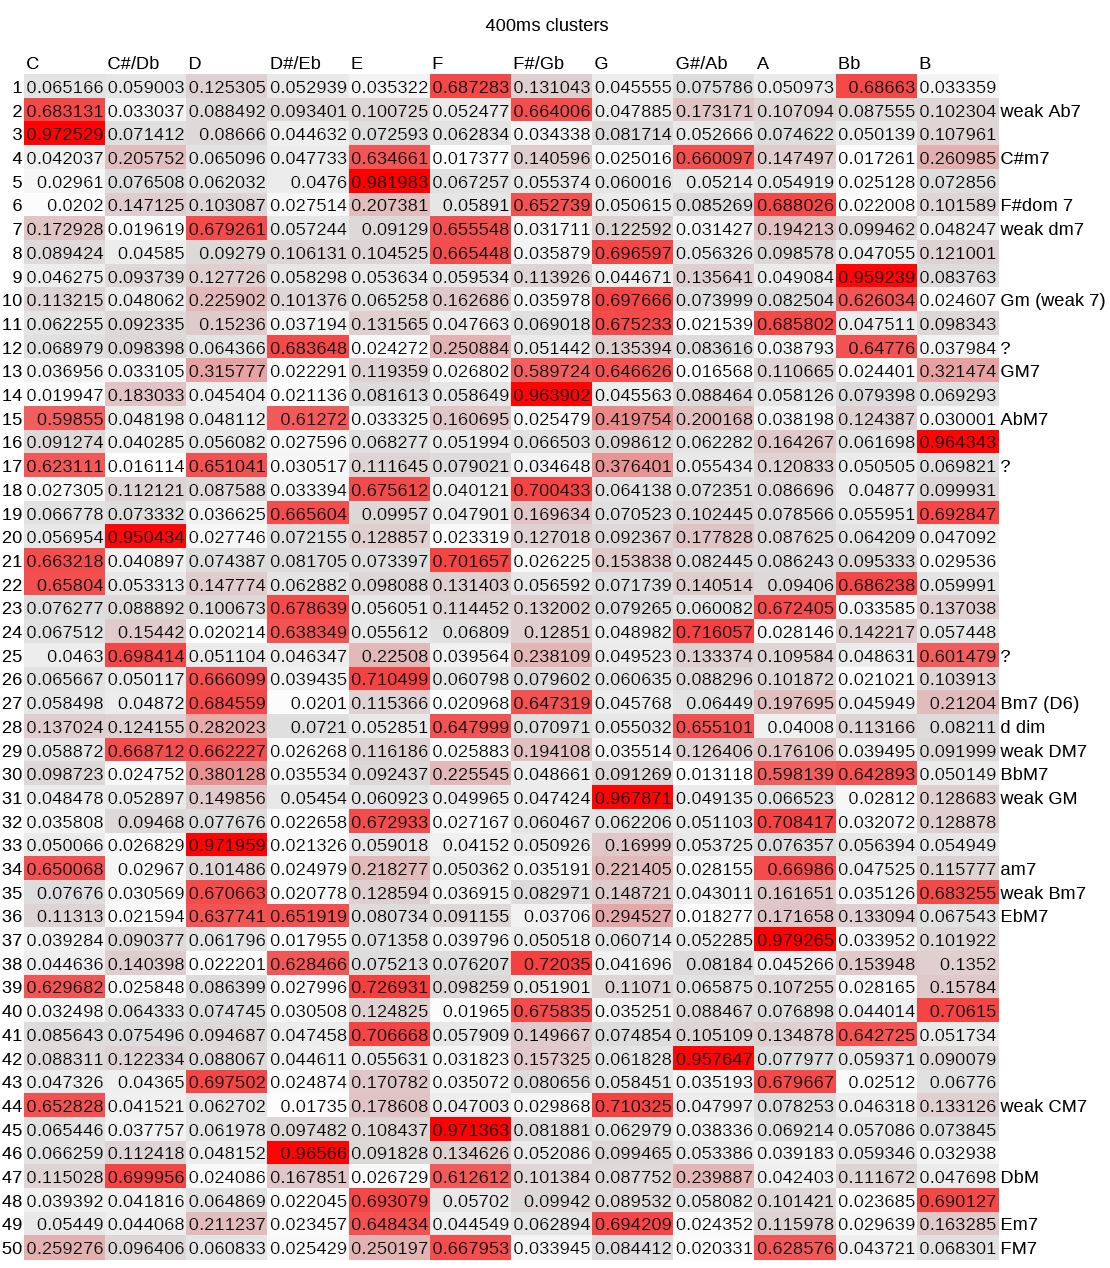
\includegraphics[width=6.5in]{400clusters.jpg}
	\caption{Spherical k-means clusters generated from durationally-weighted pc vectors corresponding to window sizes of 400ms.  Among cluster prototypes of cardinality 3 or greater, the majority correspond to traditional chord structures.}
	\label{400clusters}
\end{figure}

\begin{figure}
	\centering
	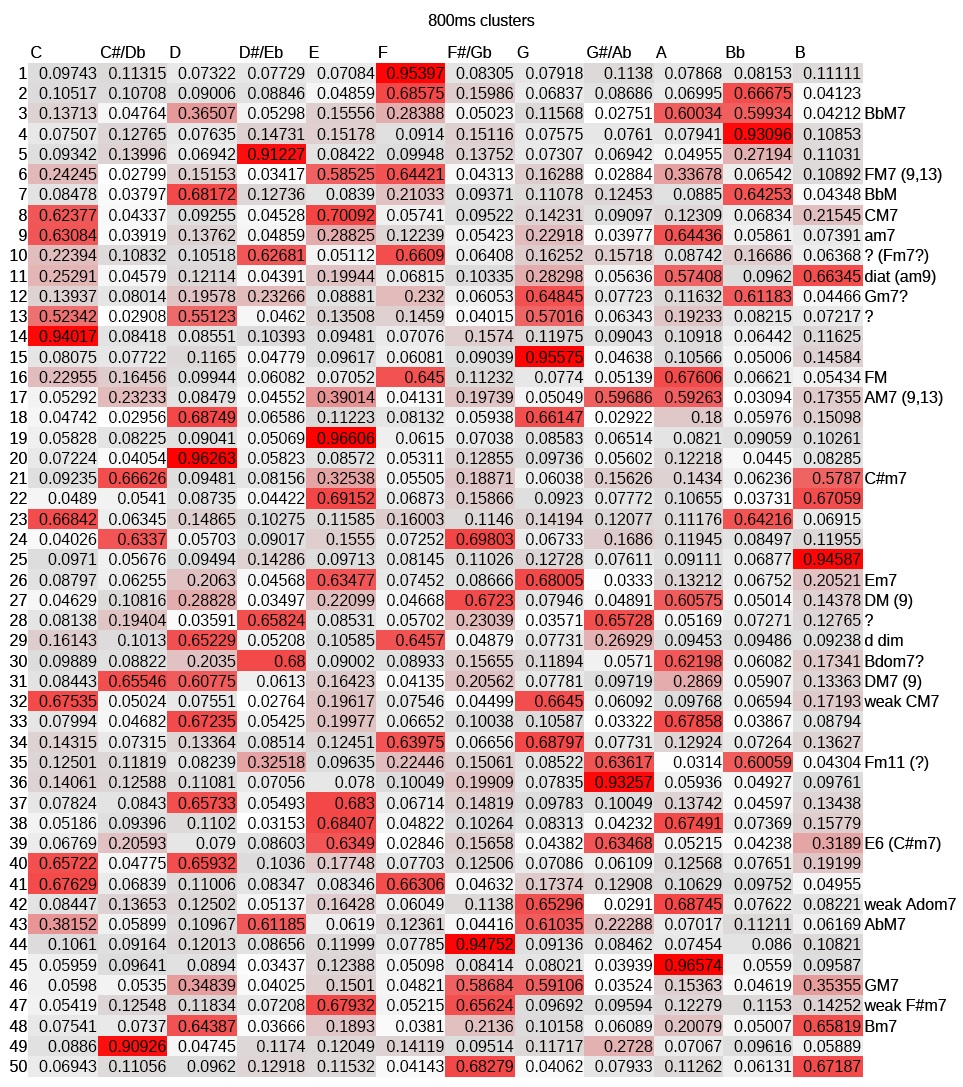
\includegraphics[width=6.5in]{800clusters.jpg}
	\caption{Spherical k-means clusters generated from durationally-weighted pc vectors corresponding to window sizes of 800ms.  The average cluster prototype cardinality is higher than the case of 400ms windows, and among those of cardinality 3 or greater, the majority correspond to traditional chord structures.}
	\label{800clusters}
\end{figure}

\begin{figure}
	\centering
	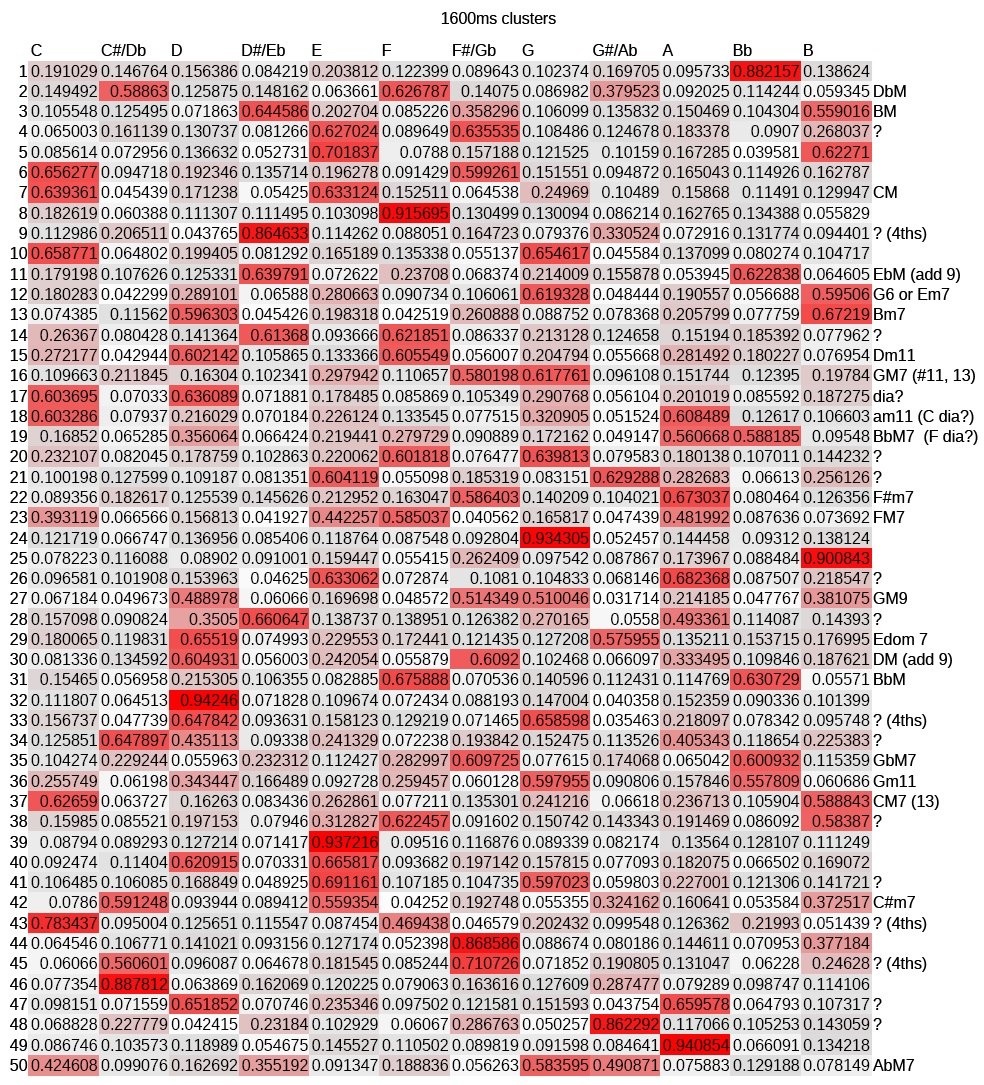
\includegraphics[width=6.5in]{1600clusters.jpg}
	\caption{Spherical k-means clusters generated from durationally-weighted pc vectors corresponding to window sizes of 1600ms.  Most cluster prototypes are of cardinality 3 or greater, and both traditionally-structured chords and potential scale fragments appear.}
	\label{1600clusters}
\end{figure}
	
